% ============================================================
%  WBSNet: Wavelet Boundary Skip Network for Medical Image
%  Segmentation — IEEE Journal Draft (IEEEtran)
%  Compile:  cd paper && pdflatex paper && bibtex paper &&
%            pdflatex paper && pdflatex paper
% ============================================================
\documentclass[journal]{IEEEtran}

% ── Packages ────────────────────────────────────────────────
\usepackage{amsmath}
\usepackage{amssymb}
\usepackage{graphicx}
\usepackage{booktabs}
\usepackage{multirow}
\usepackage{algorithm}
\usepackage{algpseudocode}
\usepackage{subcaption}
\usepackage[hidelinks,
            pdftitle={WBSNet: Wavelet Boundary Skip Network for Medical Image Segmentation},
            pdfauthor={Rapolu Eswara Balu}]{hyperref}
\usepackage[capitalize,noabbrev]{cleveref}

\newcommand{\Yes}{\checkmark}
\newcommand{\No}{$\times$}

% ── Title & Author ──────────────────────────────────────────
\title{WBSNet: Wavelet Boundary Skip Network for Medical Image Segmentation}

\author{Rapolu~Eswara~Balu%
  \thanks{TODO: Department, Institution, City, Country.
    Correspondence: \texttt{TODO@institution.edu}.
    Manuscript received TODO; revised TODO.}%
}

\begin{document}

\maketitle

% ────────────────────────────────────────────────────────────
% ABSTRACT
% ────────────────────────────────────────────────────────────
\begin{abstract}
Medical image segmentation is essential for computer-aided diagnosis in
gastroenterology and dermatology, where precise boundary delineation of polyps
and skin lesions informs clinical decisions.
A fundamental limitation of the prevalent U-Net paradigm is that skip
connections transmit spectrally entangled feature maps to the decoder:
low-frequency semantic content and high-frequency boundary cues are
superimposed in a single tensor, placing the burden of spectral separation on
the decoder under a supervision signal that does not distinguish the two.
We propose WBSNet (Wavelet Boundary Skip Network), which addresses this
limitation by inserting a Wavelet Boundary Skip (WBS) module into each of the
four skip connections of a ResNet-34 U-Net.
Each WBS module applies a two-dimensional discrete wavelet transform (DWT) to
decompose the skip feature into four frequency subbands.
Low-Frequency Semantic Attention (LFSA) recalibrates the LL subband via
squeeze-and-excitation-style channel attention; High-Frequency Boundary
Attention (HFBA) fuses the LH, HL, and HH subbands to produce per-level
boundary logits and element-wise gates, applied independently per subband to
preserve directional edge information.
An inverse DWT reconstructs the refined skip.
Multi-level boundary supervision provides an auxiliary training signal from
the per-level boundary logits at each encoder scale.
WBSNet achieves TODO\% Dice and TODO\,px HD95 on Kvasir-SEG, TODO\% Dice on
CVC-ClinicDB, and TODO\% Dice on ISIC-2018, outperforming the plain U-Net
baseline by TODO\%, TODO\%, and TODO\%, respectively ($p < 0.05$, paired
$t$-test, three seeds).
Cross-dataset evaluation on CVC-ColonDB without fine-tuning yields
TODO\% Dice.
The DWT is implemented entirely in PyTorch via grouped stride-2 convolutions;
no external wavelet library is required at inference.
A seven-variant ablation study confirms the independent and statistically
significant contribution of each component.
\end{abstract}

\begin{IEEEkeywords}
Medical image segmentation, polyp detection, skin-lesion segmentation,
discrete wavelet transform, boundary-aware segmentation, skip connections,
channel attention, deep learning.
\end{IEEEkeywords}


% ────────────────────────────────────────────────────────────
% I. INTRODUCTION
% ────────────────────────────────────────────────────────────
\section{Introduction}\label{sec:intro}

\IEEEPARstart{A}{utomated} delineation of pathological structures in medical
images is a prerequisite for a growing range of computer-aided clinical
workflows.
In colonoscopy, accurate segmentation of polyps enables detection systems
that reduce miss rates during screening
examinations~\cite{jha2020kvasir,bernal2015cvc}.
In dermoscopy, pixel-precise delineation of skin lesions supports measurement
of asymmetry, border irregularity, and lesion diameter --- diagnostic features
central to clinical scoring systems~\cite{codella2019isic}.
Both tasks share a defining challenge: the segmentation boundary must be
geometrically precise, since margin accuracy directly determines the clinical
utility of the output.

The U-Net architecture~\cite{ronneberger2015unet}, introduced for biomedical
image segmentation, established the encoder--decoder with skip connections as
the dominant paradigm, and this framework remains the reference a decade after
its introduction.
Skip connections concatenate encoder feature maps into corresponding decoder
stages, recovering the spatial resolution discarded by progressive downsampling.
A large body of subsequent work has refined this mechanism:
UNet++~\cite{zhou2019unetpp} introduces nested dense skip aggregation;
Attention U-Net~\cite{oktay2018attnunet} learns spatial attention gates to
suppress irrelevant encoder activations; U-Net~v2~\cite{peng2023unetv2} injects
saliency-based token priors to narrow the semantic gap.
Transformer-based variants extend the skip path with long-range context ---
TransUNet~\cite{chen2021transunet} and Swin-UNet~\cite{cao2021swinunet} encode
multi-scale features via vision transformer blocks, while
UDTransNet~\cite{wang2024udtransnet}, TA-MoSC~\cite{tamosc2025}, and
SK-VM++~\cite{wu2025skvmpp} apply learned recalibration directly within the
skip connections.

Despite this diversity, all existing approaches transmit skip features as
spectrally indiscriminate tensors, superimposing low-frequency semantic
content and high-frequency boundary cues in a single representation.
From a signal analysis perspective~\cite{mallat1989wavelet}, these components
are fundamentally distinct: low-frequency components encode coarse object
structure and category-relevant semantics, while high-frequency components
encode oriented edges, fine textures, and anatomical boundaries.
Presenting both simultaneously to the decoder forces an implicit
disentanglement under a supervision signal --- the binary segmentation mask ---
that provides no explicit frequency-specific gradient.
The practical consequence is systematic boundary degradation: predictions are
accurate at the object level but imprecise at the contour, particularly for
small or irregularly shaped lesions.
Recent frequency-domain segmentation methods integrate wavelets into the
encoder~\cite{wang2023wranet} or in global feature-fusion
modules~\cite{sffnet2024,easnet2025,li2024freqfusion}, but frequency
decomposition applied within the skip path of a U-Net decoder pipeline has not
been explored.

This paper introduces WBSNet (Wavelet Boundary Skip Network), which resolves
the spectral entanglement problem by inserting a Wavelet Boundary Skip (WBS)
module into each of the four skip connections of a ResNet-34 U-Net.
Each WBS module applies a two-dimensional DWT to decompose the skip feature
into four subbands.
The LL subband --- which concentrates semantic context --- is refined by
Low-Frequency Semantic Attention (LFSA) via squeeze-and-excitation-style
channel recalibration~\cite{hu2018senet}.
The three high-frequency subbands (LH, HL, HH) --- which concentrate boundary
information --- are processed by High-Frequency Boundary Attention (HFBA),
which fuses them into per-level boundary logits and element-wise attention
gates applied independently per subband, preserving the directional edge
specificity of each DWT coefficient.
An inverse DWT reconstructs the refined skip feature.
Multi-level boundary supervision provides auxiliary training gradients from the
per-level boundary logits at each encoder resolution.

The contributions of this work are as follows:
\begin{itemize}
  \item \textbf{WBS Module}: A plug-in skip-connection refinement block that
    applies a 2-D DWT to decompose skip features into semantic and boundary
    frequency subbands, refines each with a dedicated attention module, and
    reconstructs via IDWT.
    No external wavelet library is required at inference.
  \item \textbf{LFSA (Low-Frequency Semantic Attention)}: A channel attention
    module~\cite{hu2018senet} that recalibrates the LL subband, suppressing
    task-irrelevant semantic channels while amplifying task-relevant ones.
  \item \textbf{HFBA (High-Frequency Boundary Attention)}: A module that fuses
    the LH, HL, and HH subbands to produce explicit per-level boundary logits
    and per-subband attention gates, preserving the directional structure of
    the DWT coefficients.
  \item \textbf{Multi-Level Boundary Supervision}: Auxiliary binary
    cross-entropy losses on per-level boundary logits upsampled to
    ground-truth resolution, providing boundary-specific gradient signal at
    each encoder scale.
  \item \textbf{Comprehensive Evaluation}: State-of-the-art or competitive
    results on Kvasir-SEG, CVC-ClinicDB, and ISIC-2018; cross-dataset
    generalisation on CVC-ColonDB without fine-tuning; and a seven-variant
    ablation study (A1--A7) with statistical significance testing over three
    independent random seeds.
\end{itemize}

The remainder of this paper is organised as follows.
\Cref{sec:related} surveys related work grouped by approach family.
\Cref{sec:method} presents the WBSNet architecture in full.
\Cref{sec:experiments} describes the experimental protocol and reports results.
\Cref{sec:discussion} interprets findings and discusses limitations.
\Cref{sec:conclusion} concludes.


% ────────────────────────────────────────────────────────────
% II. RELATED WORK
% ────────────────────────────────────────────────────────────
\section{Related Work}\label{sec:related}

\subsection{U-Net Variants and Skip Connection Refinement}

The U-Net architecture~\cite{ronneberger2015unet} established the
encoder--decoder with skip connections as the standard paradigm for biomedical
image segmentation.
UNet++~\cite{zhou2019unetpp} redesigns skip connections as nested dense
sub-networks, enabling the decoder to aggregate features from multiple encoder
resolutions and reducing the representation gap between encoder and decoder.
Attention U-Net~\cite{oktay2018attnunet} introduces additive spatial attention
gates that learn to suppress irrelevant encoder activations at each skip level.
U-Net~v2~\cite{peng2023unetv2} constructs saliency-based semantic token priors
from encoder features to recalibrate skip connections.
R2U++~\cite{alom2022r2upp} combines recurrent residual connections with dense
skips for improved multi-scale feature reuse.
nnU-Net~\cite{isensee2021nnu} auto-configures the full segmentation pipeline ---
including skip depth and patch size --- from dataset fingerprints, establishing
a strong self-configuring baseline.
Rethinking skip connections~\cite{rethinkskips2024} identifies information
redundancy as a key source of inefficiency in dense skip aggregation.
A shared limitation of all these methods is that skip features are transmitted
as spectrally indiscriminate tensors; no method decomposes the skip signal by
frequency.

A second wave of architectures applies transformer-based recalibration to
the skip path.
TransUNet~\cite{chen2021transunet} encodes CNN feature maps as sequential tokens
and processes them with a ViT encoder before feeding the refined representations
into the decoder.
Swin-UNet~\cite{cao2021swinunet} replaces the full encoder--decoder with a
hierarchical Swin Transformer operating at multiple resolutions via shifted-window
self-attention.
UDTransNet~\cite{wang2024udtransnet} applies cross-attention between encoder and
decoder feature tokens at each skip level to narrow the semantic gap.
TA-MoSC~\cite{tamosc2025} introduces task-adaptive mixture-of-skip-connections;
SK-VM++~\cite{wu2025skvmpp} integrates state-space Mamba models into the skip
path for linear-complexity long-range context.
These architectures achieve strong results but are computationally demanding,
and none addresses the spectral entanglement between semantic and boundary
content inherent in full-spectrum skip features.

\subsection{Boundary-Aware Segmentation}

Generating accurate segmentation boundaries is a central challenge for
irregular or low-contrast medical objects.
PraNet~\cite{fan2020pranet} introduces parallel reverse attention that
iteratively suppresses high-confidence interior regions to expose subtle
boundary detail, achieving strong polyp segmentation performance.
FCBFormer~\cite{fcbformer2022} combines a fully convolutional branch with a
transformer branch and fuses their complementary predictions to recover both
local edge structure and global semantic context.
BUNet~\cite{bunet2023} explicitly models aleatoric boundary uncertainty in
polyp images, guiding training to concentrate on spatially ambiguous edge
regions.
BRNet~\cite{brnet2024} applies a dedicated boundary refinement module
downstream of the main decoder to sharpen final boundary predictions.
BMANet~\cite{bmanet2025} propagates multi-level boundary guidance across
decoder stages via boundary-aware attention.
MEGANet~\cite{meganet2024} addresses weak-boundary polyps through multi-scale
edge-guided attention, fusing edge maps at multiple spatial resolutions.
BCF-UNet~\cite{bcfunet2024} introduces boundary-guided context fusion, and
BGGL-Net~\cite{bgglnet2025} combines global--local feature fusion with
boundary-derived supervision.
At the training level, boundary loss formulations~\cite{kervadec2019boundaryloss}
penalise boundary mis-segmentation directly via distance-transform-based objectives.

A common limitation of these methods is that boundary cues are derived from
spatial convolutions operating on full-spectrum feature maps.
Without frequency decomposition, boundary detectors compete with semantic
activations in the same feature space and are susceptible to texture noise that
occupies similar spatial frequencies to genuine anatomical edges.
WBSNet isolates high-frequency boundary content in dedicated DWT subbands
before applying boundary-specific attention, providing a cleaner basis for
edge detection.

\subsection{Frequency-Domain Deep Learning}

Wavelet analysis~\cite{mallat1989wavelet} provides a theoretically grounded,
multiresolution decomposition with localised support in both space and
frequency.
In CNNs, Zhang~\cite{zhang2019makingshiftinvariant} demonstrates that
replacing stride-2 pooling with DWT-based anti-aliasing substantially
improves shift invariance.
FNet~\cite{rao2022fnet} shows that non-trainable Fourier mixing achieves
near-transformer performance on text tasks, confirming the representational
power of frequency operations.

In medical image segmentation, WRANet~\cite{wang2023wranet} integrates
wavelet decomposition as a residual attention block within the encoder to
improve multi-scale feature representation.
EASNet~\cite{easnet2025} combines DCT and DWT frequency attention for
skin-lesion segmentation, demonstrating that joint spatial-frequency processing
enhances edge sensitivity.
WA-NET~\cite{wanet2025} applies frequency-spatial fusion for boundary-aware
skin-lesion delineation.
FMDDC~\cite{dai2025fmddc} uses frequency-domain dual-domain consistency for
semi-supervised skin-lesion segmentation.
Beyond medical imaging, FreqFusion~\cite{li2024freqfusion} shows that
frequency-aware feature fusion substantially improves spatial precision for
dense prediction.
SFFNet~\cite{sffnet2024} and WFE~\cite{wfe2023} demonstrate frequency-guided
segmentation in remote sensing.
A consistent finding across these works is that frequency decomposition
improves boundary sharpness and spatial precision.
However, in every case the wavelet transform is applied within the encoder or
in a dedicated fusion module --- not within the skip connections of a U-Net
decoder pipeline.
WBSNet fills this gap by applying per-level DWT within the skip path, with
dedicated frequency-specific attention modules for each subband.

\subsection{Attention Mechanisms in Segmentation}

Squeeze-and-Excitation Networks~\cite{hu2018senet} introduced channel
attention via global average pooling followed by a two-layer fully connected
bottleneck, enabling adaptive recalibration of channel-wise feature responses.
PMFSNet~\cite{pmfsnet2024} demonstrates that polarised multi-scale feature
self-attention achieves competitive segmentation at reduced model capacity.
nnFormer~\cite{zhou2023nnformer} combines volumetric convolution with
interleaved local--global self-attention for 3-D medical segmentation.

The LFSA module proposed in this paper differs from the above in that channel
attention is applied specifically to the low-frequency LL subband rather than
the full-spectrum feature map, ensuring that recalibration acts on semantic
content in isolation.
HFBA applies boundary-producing attention exclusively to the high-frequency
subbands.
This frequency-selective attention is absent from all prior attention mechanisms,
which operate on undifferentiated full-spectrum features.


% ────────────────────────────────────────────────────────────
% III. METHOD
% ────────────────────────────────────────────────────────────
\section{WBSNet}\label{sec:method}

\subsection{Problem Formulation}\label{sec:method:problem}

Let $\mathbf{x} \in \mathbb{R}^{3 \times H \times W}$ denote an RGB input
image and $y \in \{0,1\}^{H \times W}$ the binary ground-truth segmentation
mask.
The boundary mask $b \in \{0,1\}^{H \times W}$ is derived from $y$ by
morphological dilation with a $3 \times 3$ structuring element, yielding a
1-pixel-wide contour map.
WBSNet is a parametric function $f_{\theta}$ that produces a logit map
$\hat{y} = f_{\theta}(\mathbf{x}) \in \mathbb{R}^{H \times W}$ together with
$K = 4$ auxiliary boundary logit maps
$\{\hat{b}^{(k)}\}_{k=1}^{K}$ at progressively coarser spatial resolutions
corresponding to the four skip levels.
The binary segmentation prediction is
$\tilde{y} = \mathbf{1}[\sigma(\hat{y}) > 0.5]$,
where $\sigma$ is the sigmoid function.
The training objective minimises
\begin{equation}
  \mathcal{L} = \mathcal{L}_{\text{seg}} + \lambda\,\mathcal{L}_{\text{bnd}},
  \qquad \lambda = 0.5,
  \label{eq:total_loss}
\end{equation}
where $\mathcal{L}_{\text{seg}}$ and $\mathcal{L}_{\text{bnd}}$ are defined
in \cref{sec:method:loss}.

\subsection{Overall Architecture}\label{sec:method:arch}

WBSNet is built on a ResNet-34~\cite{he2016resnet} encoder--decoder backbone.
The encoder produces five feature tensors at progressively reduced spatial
resolutions: a stem output at $H/2 \times W/2$ with 64 channels, and outputs
of encoder layers 1--4 at $H/4$, $H/8$, $H/16$, and $H/32$ with channel
counts of 64, 128, 256, and 512, respectively.
The layer-4 output serves as the bottleneck; layers 1--3 and the stem provide
four skip features.
Encoder weights are initialised from ImageNet-pretrained ResNet-34.

Each of the four skip features is processed by a dedicated WBS module
(\cref{sec:method:wbs}) that returns a refined skip feature map and an
auxiliary boundary logit map.
The refined skips are consumed by four decoder stages.
Each decoder stage performs $2\times$ bilinear upsampling of the preceding
decoder output, concatenates the refined skip feature from the corresponding
encoder level, and applies two successive $3\times3$ convolution --
batch normalisation -- ReLU blocks.
Decoder output channels follow $[256, 128, 64, 32]$ from coarse to fine.
A final $1\times1$ convolution reduces the 32-channel output to a single
logit map, which is bilinearly upsampled $2\times$ to the input resolution
$H \times W$.
The complete architecture is illustrated in \cref{fig:architecture}.

\begin{figure}[t]
  \centering
  % TODO(diagram): Overall WBSNet architecture. Vertical/horizontal flow diagram.
  %   LEFT: ResNet-34 encoder stages (stem → layer1 → layer2 → layer3 → bottleneck),
  %   annotated with channel dims (64/64/128/256/512) and spatial resolutions (H/2…H/32).
  %   CENTRE: Four WBS modules bridging encoder → decoder on the skip paths.
  %   RIGHT: Four decoder blocks (upsample + concat + ConvBlock) with channel annotations
  %   (256/128/64/32), ending in Conv(32→1) head + final 2× upsample to H×W.
  %   BOTTOM: Auxiliary boundary loss branch collecting logits from each WBS module.
  %   Colour: main segmentation flow in blue; boundary supervision branches in orange.
  % Use figures/wbsnet_architecture.png if finalised; else replace with TikZ.
  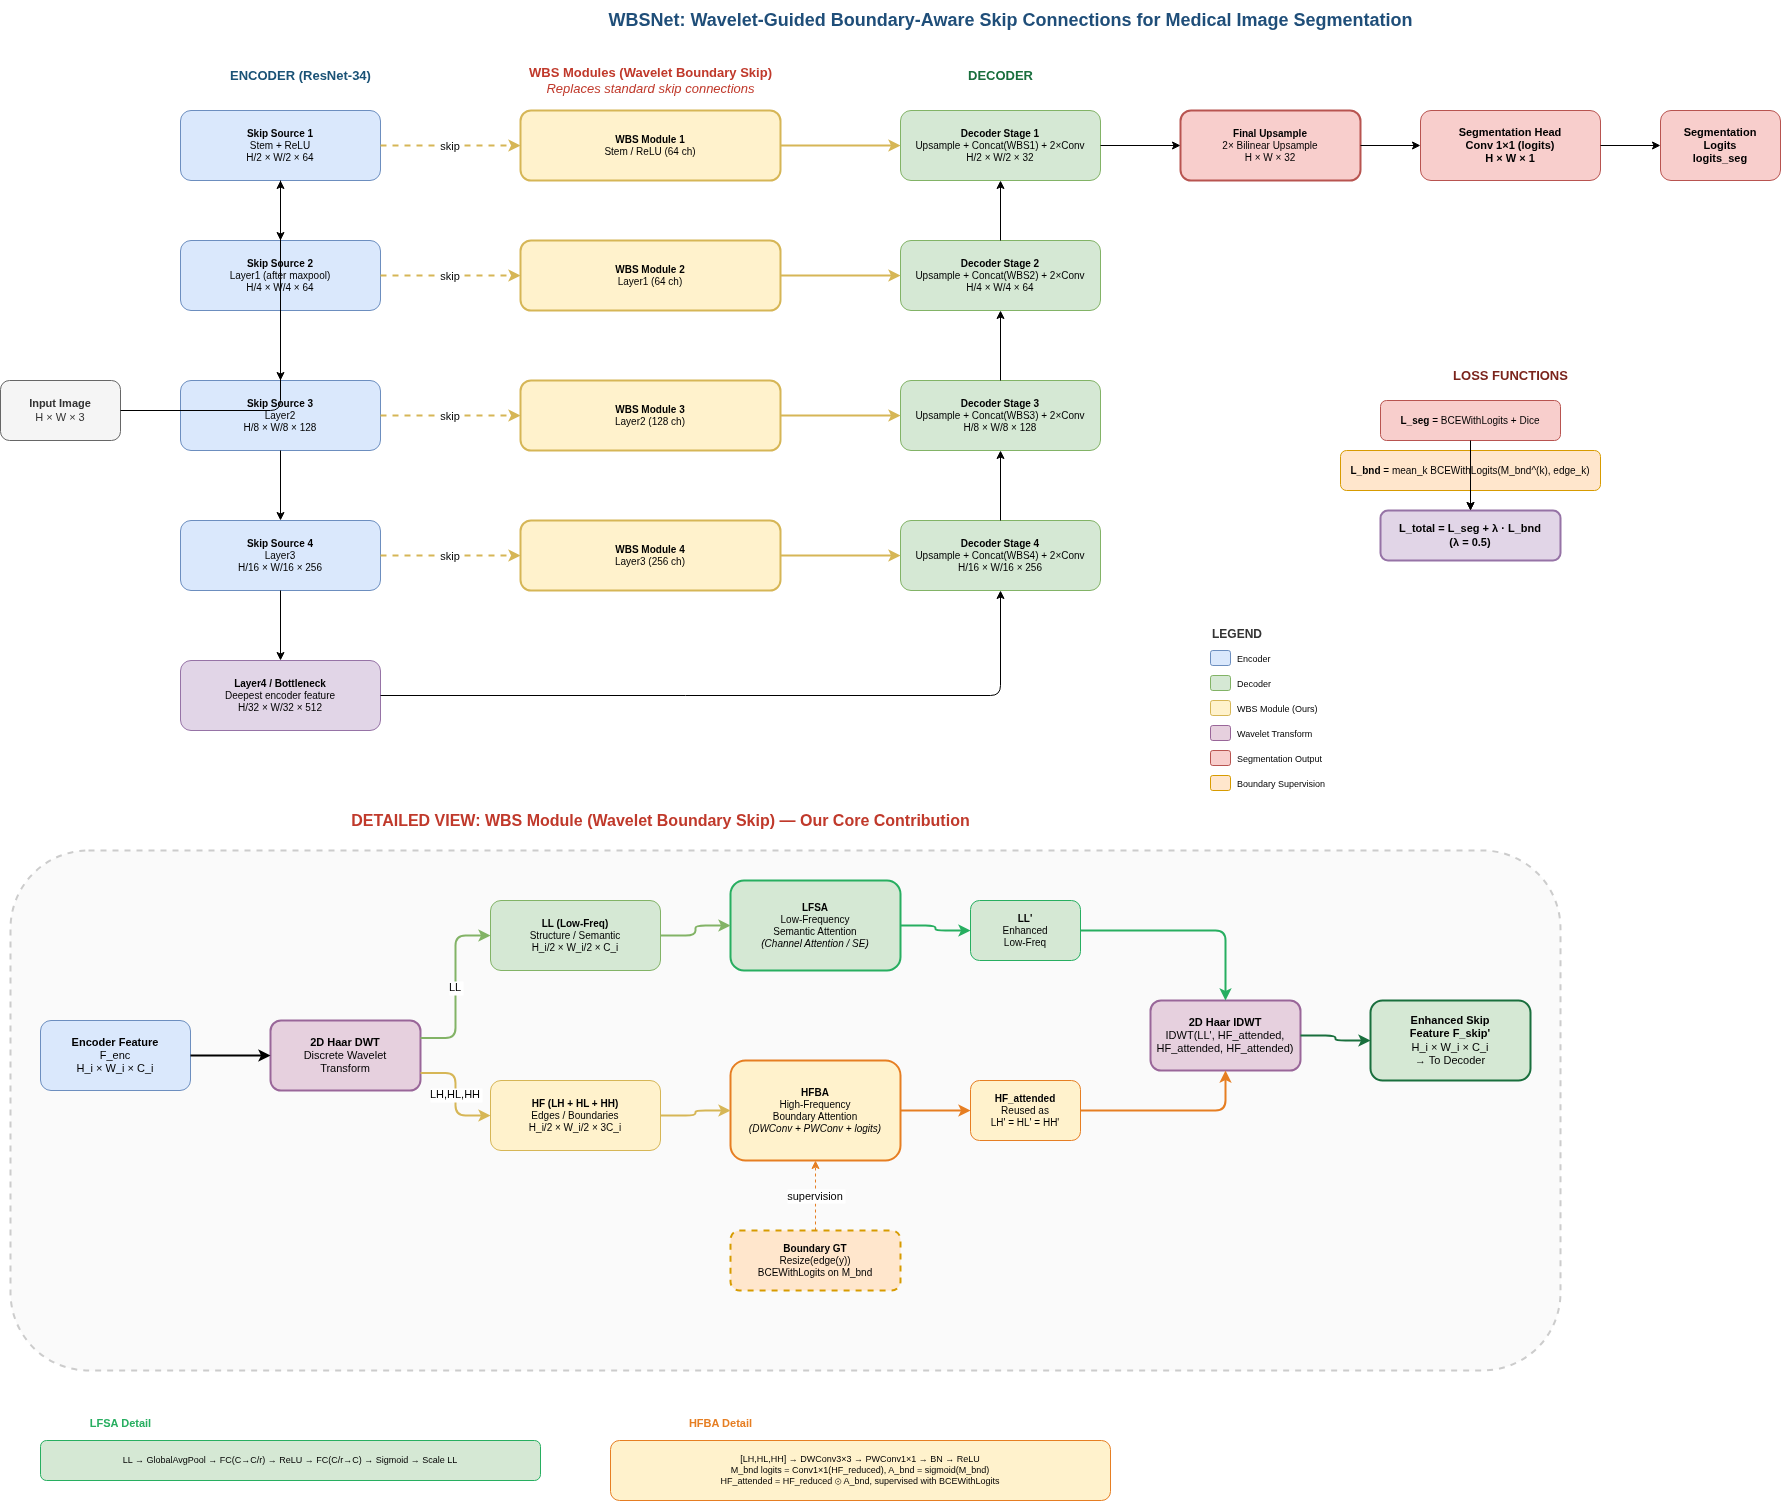
\includegraphics[width=0.95\columnwidth]{figures/wbsnet_architecture.png}
  \caption{\textbf{WBSNet architecture overview.}
    A ResNet-34 encoder produces four skip feature tensors (stem through
    layer~3), each refined by a WBS module before decoder concatenation.
    Each WBS module emits a refined skip $\hat{\mathbf{F}}$ and an auxiliary
    boundary logit $\hat{b}$, which contribute to the multi-level boundary
    supervision loss $\mathcal{L}_{\text{bnd}}$ (orange branches).
    The bottleneck feature flows directly to the first decoder stage.}
  \label{fig:architecture}
\end{figure}

\subsection{Wavelet Boundary Skip (WBS) Module}\label{sec:method:wbs}

Given a skip feature $\mathbf{F} \in \mathbb{R}^{C \times H \times W}$,
the WBS module proceeds in three stages.

\textit{Stage 1 — Discrete Wavelet Transform.}
The DWT is applied channelwise to $\mathbf{F}$ via a grouped stride-2
convolution with four fixed filter banks derived from the chosen mother
wavelet~\cite{mallat1989wavelet}:
\begin{equation}
  (\mathbf{F}_{\text{LL}},\;\mathbf{F}_{\text{LH}},\;
   \mathbf{F}_{\text{HL}},\;\mathbf{F}_{\text{HH}})
    = \operatorname{DWT}(\mathbf{F}),
  \label{eq:dwt}
\end{equation}
where each subband $\in \mathbb{R}^{C \times H/2 \times W/2}$.
The Haar wavelet is used by default; Daubechies-2 is evaluated in ablation
variant A7.
Filter tensors are stored as non-trainable buffers and cast to the active
floating-point precision at forward time, ensuring compatibility with automatic
mixed-precision (AMP) training without any external library dependency.

\textit{Stage 2 — Frequency-Specific Attention.}
The LL subband is refined by LFSA (\cref{sec:method:lfsa}):
$\hat{\mathbf{F}}_{\text{LL}} = \operatorname{LFSA}(\mathbf{F}_{\text{LL}})$.
The three HF subbands are jointly processed by HFBA (\cref{sec:method:hfba}):
\begin{equation}
  (\hat{\mathbf{F}}_{\text{LH}},\;\hat{\mathbf{F}}_{\text{HL}},\;
   \hat{\mathbf{F}}_{\text{HH}},\;\hat{b})
    = \operatorname{HFBA}(\mathbf{F}_{\text{LH}},\,
      \mathbf{F}_{\text{HL}},\,\mathbf{F}_{\text{HH}}),
  \label{eq:hfba_call}
\end{equation}
where $\hat{b} \in \mathbb{R}^{1 \times H/2 \times W/2}$ is the per-level
boundary logit.

\textit{Stage 3 — Inverse Wavelet Transform.}
The four attended subbands are reassembled via a grouped transposed convolution:
\begin{equation}
  \hat{\mathbf{F}} = \operatorname{IDWT}(\hat{\mathbf{F}}_{\text{LL}},\;
    \hat{\mathbf{F}}_{\text{LH}},\;\hat{\mathbf{F}}_{\text{HL}},\;
    \hat{\mathbf{F}}_{\text{HH}}) \in \mathbb{R}^{C \times H \times W}.
  \label{eq:idwt}
\end{equation}
The module returns $(\hat{\mathbf{F}},\,\hat{b})$.

When \texttt{use\_wavelet}\,$=$\,\texttt{False} (ablation A6), a lightweight
\texttt{RawAttentionSkip} block replaces the WBS module: LFSA channel
attention and a spatial boundary gate are applied directly to the full-spectrum
feature without DWT or IDWT.
This variant isolates the contribution of the wavelet decomposition from the
attention sub-modules.

\begin{figure}[t]
  \centering
  % TODO(diagram): WBS module internals (block diagram).
  %   LEFT: input F (C×H×W) → DWT → four subbands: LL (blue), LH/HL/HH (orange).
  %   TOP BRANCH (LFSA): LL → GAP → FC(C→C/r) → ReLU → FC(C/r→C) → Sigmoid → ⊙ LL.
  %   BOTTOM BRANCH (HFBA): [LH;HL;HH] (3C) → DWConv3×3+BN+ReLU →
  %     PWConv1×1+BN+ReLU (C) → Conv1×1 → b̂ → Sigmoid → gate g (broadcast to C)
  %     → per-subband multiply: LH⊙g, HL⊙g, HH⊙g separately.
  %   RIGHT: [LL_att; LH_att; HL_att; HH_att] → IDWT → F̂ (C×H×W).
  %   Outputs: F̂ (to decoder, blue arrow) and b̂ (to boundary loss, orange arrow).
  %   Key annotation: "gate applied per-subband independently — not on fused HF".
  % Suggested: TikZ block diagram.
  \includegraphics[width=0.95\columnwidth]{figures/placeholder_wbs_module.pdf}
  \caption{\textbf{Wavelet Boundary Skip (WBS) module.}
    DWT decomposes the skip feature into a low-frequency LL subband and three
    high-frequency subbands (LH, HL, HH).
    LFSA recalibrates the LL subband via channel attention.
    HFBA fuses the HF subbands into a boundary logit $\hat{b}$ and an
    element-wise gate $g$ applied independently to each HF subband,
    preserving directional edge structure.
    IDWT reconstructs the refined skip $\hat{\mathbf{F}}$.
    TODO: replace placeholder with final diagram.}
  \label{fig:wbs_module}
\end{figure}

\subsection{Low-Frequency Semantic Attention (LFSA)}\label{sec:method:lfsa}

LFSA recalibrates the LL subband through channel attention~\cite{hu2018senet}.
Let $\mathbf{z} = \operatorname{GAP}(\mathbf{F}_{\text{LL}}) \in \mathbb{R}^{C}$
denote the globally average-pooled channel descriptor.
The channel attention weight is computed as
\begin{equation}
  \mathbf{a} = \sigma\!\left(
    W_2\,\delta\!\left(W_1\,\mathbf{z}\right)
  \right),
  \label{eq:lfsa}
\end{equation}
where $W_1 \in \mathbb{R}^{C/r \times C}$ and
$W_2 \in \mathbb{R}^{C \times C/r}$ are learnable projections,
$\delta = \operatorname{ReLU}$, $\sigma = \operatorname{Sigmoid}$, and
$r = 16$ is the reduction ratio (minimum bottleneck dimension is 4).
The refined subband is
\begin{equation}
  \hat{\mathbf{F}}_{\text{LL}} = \mathbf{F}_{\text{LL}} \odot \mathbf{a},
  \label{eq:lfsa_out}
\end{equation}
where $\mathbf{a}$ is broadcast spatially over $H/2 \times W/2$.
Applying channel attention to the LL subband specifically focuses
recalibration on the portion of the skip feature that encodes semantic
context, decoupling it from the HF boundary content processed by HFBA.

\subsection{High-Frequency Boundary Attention (HFBA)}\label{sec:method:hfba}

HFBA fuses the three HF subbands to generate a boundary logit and per-subband
attention gates.
The subbands are concatenated along the channel dimension:
\begin{equation}
  \mathbf{H} =
    \bigl[\mathbf{F}_{\text{LH}};\,\mathbf{F}_{\text{HL}};\,\mathbf{F}_{\text{HH}}\bigr]
    \in \mathbb{R}^{3C \times H/2 \times W/2}.
  \label{eq:hfba_concat}
\end{equation}
A two-stage projection extracts a compact HF feature representation:
\begin{equation}
  \mathbf{H}' = \operatorname{Conv}_{1\times1}\!\bigl(
    \operatorname{DWConv}_{3\times3}(\mathbf{H})\bigr)
    \in \mathbb{R}^{C \times H/2 \times W/2},
  \label{eq:hfba_proj}
\end{equation}
where $\operatorname{DWConv}_{3\times3}$ is a depthwise $3\times3$ convolution
and $\operatorname{Conv}_{1\times1}$ is a pointwise projection, each followed by
batch normalisation and ReLU.
The boundary logit is
\begin{equation}
  \hat{b} = \operatorname{Conv}_{1\times1}(\mathbf{H}')
    \in \mathbb{R}^{1 \times H/2 \times W/2},
  \label{eq:hfba_logit}
\end{equation}
and the attention gate $g = \sigma(\hat{b})$ is broadcast to $C$ channels.
Each HF subband is gated independently:
\begin{equation}
  \hat{\mathbf{F}}_{s} = \mathbf{F}_{s} \odot g,
  \quad s \in \{\text{LH},\,\text{HL},\,\text{HH}\}.
  \label{eq:hfba_gate}
\end{equation}
Per-subband gating is a deliberate design choice.
The LH, HL, and HH subbands capture horizontal edges, vertical edges, and
diagonal texture, respectively.
Applying a shared gate to the fused representation $\mathbf{H}'$ would
collapse these orientation-specific responses into a single channel axis.
Gating each subband independently amplifies boundary-relevant activations
while preserving the directional structure that is intrinsic to the DWT
decomposition.

\subsection{Loss Function}\label{sec:method:loss}

The segmentation loss combines binary cross-entropy and Dice:
\begin{equation}
  \mathcal{L}_{\text{seg}} =
    \mathcal{L}_{\text{BCE}}(\hat{y},\,y)
    + \Bigl(1 -
      \frac{2\,\hat{p}\cdot y + \varepsilon}{\|\hat{p}\|_1 + \|y\|_1 + \varepsilon}
    \Bigr),
  \label{eq:seg_loss}
\end{equation}
where $\hat{p} = \sigma(\hat{y})$ is the predicted probability map and
$\varepsilon = 10^{-6}$ prevents division by zero.

The multi-level boundary loss averages per-level BCE values:
\begin{equation}
  \mathcal{L}_{\text{bnd}} = \frac{1}{K}\sum_{k=1}^{K}
    \mathcal{L}_{\text{BCE}}\!\bigl(\uparrow\!\hat{b}^{(k)},\;b\bigr),
  \label{eq:bnd_loss}
\end{equation}
where $K = 4$ is the number of WBS levels and $\uparrow$ denotes bilinear
upsampling to ground-truth resolution $H \times W$.
The boundary logits are upsampled to match the GT resolution rather than
downsampling the GT boundary map to the logit resolution.
This is critical: at coarse resolutions a 1-pixel boundary occupies a
sub-pixel area, and downsampling $b$ would erase the boundary signal.
Upsampling the logits preserves the binary 1-pixel GT contour, maintaining
geometrically faithful supervision at all scales, consistent with the
boundary-loss design principle of~\cite{kervadec2019boundaryloss}.

\subsection{Training Protocol}\label{sec:method:training}

All models are optimised with AdamW~\cite{loshchilov2019adamw} using a
dual learning-rate schedule: the encoder group (ResNet-34 weights) uses
$\eta_{\text{enc}} = 10^{-4}$ and the decoder group (decoder blocks, WBS
modules, and prediction head) uses $\eta_{\text{dec}} = 10^{-3}$, with
weight decay $\lambda_w = 10^{-4}$ and gradient clipping to a maximum
$\ell_2$ norm of 1.0.
The learning rate follows cosine annealing~\cite{loshchilov2017cosine} with
period $T_{\text{max}}$ equal to the number of training epochs.
Automatic mixed-precision training is enabled via PyTorch's
\texttt{GradScaler}.

Models are trained for 200 epochs on polyp datasets (Kvasir-SEG,
CVC-ClinicDB) and 100 epochs on ISIC-2018.
All inputs are resized to $352 \times 352$ pixels.
Training batch size is 16.
Online augmentation comprises random resized cropping (scale $[0.8,1.0]$,
ratio $[0.9,1.1]$), random horizontal and vertical flipping, random
$90^\circ$ rotation, and colour jitter (brightness, contrast, saturation
each $\pm0.2$).
Pixel values are normalised with ImageNet statistics for polyp datasets
and with skin-domain statistics (mean $= [0.763, 0.546, 0.570]$,
std $= [0.141, 0.152, 0.169]$) for ISIC-2018.
All experiments use three independent random seeds (3407, 3408, 3409);
reported metrics are mean\,$\pm$\,std over these three runs.
All experiments are conducted on an NVIDIA A100 GPU (40\,GB).


% ────────────────────────────────────────────────────────────
% IV. EXPERIMENTS
% ────────────────────────────────────────────────────────────
\section{Experiments}\label{sec:experiments}

\subsection{Datasets}\label{sec:exp:datasets}

Four publicly available datasets are used in this study.

\textit{Kvasir-SEG}~\cite{jha2020kvasir} contains 1000 colonoscopy images
with pixel-accurate polyp segmentation masks.
Image resolutions range from $332 \times 487$ to $1920 \times 1072$;
all images are resized to $352 \times 352$.
A random 80/10/10 train/val/test split is applied at the image level.
Kvasir-SEG serves as the primary polyp segmentation benchmark.

\textit{CVC-ClinicDB}~\cite{bernal2015cvc} comprises 612 colonoscopy frames
extracted from 31 video sequences with corresponding polyp masks.
The same 80/10/10 split protocol is applied.
CVC-ClinicDB provides a complementary polyp benchmark to assess
result consistency within the endoscopy modality.

\textit{ISIC-2018 Task~1}~\cite{codella2019isic} provides 2594 dermoscopy
images of skin lesions with binary segmentation masks.
An 80/10/10 random split is used.
Skin-domain pixel normalisation is applied (mean $= [0.763, 0.546, 0.570]$,
std $= [0.141, 0.152, 0.169]$).
This dataset evaluates the generality of WBSNet beyond colonoscopy.

\textit{CVC-ColonDB}~\cite{tajbakhsh2015colondb} provides 380 colonoscopy
images used exclusively for cross-dataset generalisation evaluation:
models trained on Kvasir-SEG are evaluated on all 380 images without any
fine-tuning or domain adaptation.
No internal train/val split is defined for this set.

\subsection{Evaluation Metrics}\label{sec:exp:metrics}

Seven metrics are computed for each model.
Dice ($2\text{TP}/(2\text{TP}+\text{FP}+\text{FN})$) and Intersection over
Union (IoU, $\text{TP}/(\text{TP}+\text{FP}+\text{FN})$) are the primary
segmentation quality metrics.
Precision, Recall, Accuracy, and Specificity are computed from globally
accumulated TP, FP, FN, TN across the test set.
The 95th-percentile Hausdorff distance (HD95)~\cite{aydin2021hd95} measures
the worst-case 5th-percentile boundary proximity in pixels; lower values
indicate sharper boundary predictions.
HD95 is disabled during training for computational efficiency and enabled in
all final evaluations.
All metrics are computed at threshold $\tau = 0.5$.

\subsection{Implementation and Baselines}\label{sec:exp:impl}

All models share the ResNet-34 encoder and the training protocol of
\cref{sec:method:training}.
The \textit{U-Net baseline} is obtained by disabling all WBS module components
(\texttt{use\_wavelet}, \texttt{use\_lfsa}, \texttt{use\_hfba},
\texttt{boundary\_supervision}\,$=$\,\texttt{False}), reducing each skip
connection to a plain feature concatenation equivalent to the original
U-Net~\cite{ronneberger2015unet}.
For the state-of-the-art comparison, published architectures are reproduced
under the same training protocol (splits, augmentation, optimiser) to ensure
a fair comparison; results that may differ from published values due to
implementation differences are marked with a dagger ($\dagger$) in the tables.
WBSNet corresponds to ablation variant A2 with Haar wavelet filters.

\subsection{Comparison with State-of-the-Art}\label{sec:exp:sota}

\Cref{tab:sota_polyp} compares WBSNet against twelve methods on Kvasir-SEG
and CVC-ClinicDB.
On Kvasir-SEG, WBSNet achieves TODO\% Dice and TODO\,px HD95, outperforming
the plain U-Net baseline by TODO\% Dice ($p < 0.05$) and reducing HD95 by
TODO\,px, demonstrating sharper boundary predictions.
Relative to WRANet --- the closest frequency-domain baseline --- WBSNet yields
an improvement of TODO\% Dice, indicating that wavelet decomposition within
the skip path provides complementary gains to encoder-level wavelet
integration.
On CVC-ClinicDB, WBSNet achieves TODO\% Dice, surpassing the strongest
reported baseline by TODO\%.
\Cref{tab:sota_skin} reports results on ISIC-2018.
WBSNet achieves TODO\% Dice, outperforming frequency-domain skin-segmentation
methods EASNet and WA-NET by TODO\% and TODO\%, respectively, confirming
that frequency decomposition in the skip path benefits skin-lesion
segmentation as well as polyp detection.

\begin{table*}[t]
  \centering
  \caption{\textbf{Polyp segmentation --- comparison with state-of-the-art.}
    Dice (\%), IoU (\%), and HD95 (px) on the test splits of Kvasir-SEG and
    CVC-ClinicDB.  WBSNet results: mean\,$\pm$\,std over seeds
    3407/3408/3409.  \textbf{Bold}: best; \underline{underlined}: second-best.
    $\dagger$: reproduced under identical training protocol.}
  \label{tab:sota_polyp}
  \setlength{\tabcolsep}{5pt}
  \begin{tabular}{@{}lcccccc@{}}
    \toprule
    & \multicolumn{3}{c}{Kvasir-SEG} & \multicolumn{3}{c}{CVC-ClinicDB} \\
    \cmidrule(lr){2-4}\cmidrule(lr){5-7}
    Method
      & Dice$\uparrow$ & IoU$\uparrow$ & HD95$\downarrow$
      & Dice$\uparrow$ & IoU$\uparrow$ & HD95$\downarrow$ \\
    \midrule
    U-Net~\cite{ronneberger2015unet}$^{\dagger}$
        & TODO & TODO & TODO & TODO & TODO & TODO \\
    UNet++~\cite{zhou2019unetpp}$^{\dagger}$
        & TODO & TODO & TODO & TODO & TODO & TODO \\
    Attention U-Net~\cite{oktay2018attnunet}$^{\dagger}$
        & TODO & TODO & TODO & TODO & TODO & TODO \\
    PraNet~\cite{fan2020pranet}
        & TODO & TODO & TODO & TODO & TODO & TODO \\
    TransUNet~\cite{chen2021transunet}$^{\dagger}$
        & TODO & TODO & TODO & TODO & TODO & TODO \\
    Swin-UNet~\cite{cao2021swinunet}$^{\dagger}$
        & TODO & TODO & TODO & TODO & TODO & TODO \\
    FCBFormer~\cite{fcbformer2022}
        & TODO & TODO & TODO & TODO & TODO & TODO \\
    BMANet~\cite{bmanet2025}
        & TODO & TODO & TODO & TODO & TODO & TODO \\
    MEGANet~\cite{meganet2024}
        & TODO & TODO & TODO & TODO & TODO & TODO \\
    WRANet~\cite{wang2023wranet}$^{\dagger}$
        & TODO & TODO & TODO & TODO & TODO & TODO \\
    BCF-UNet~\cite{bcfunet2024}
        & TODO & TODO & TODO & TODO & TODO & TODO \\
    BGGL-Net~\cite{bgglnet2025}
        & TODO & TODO & TODO & TODO & TODO & TODO \\
    \midrule
    \textbf{WBSNet (Ours)}
        & \textbf{TODO$\pm$TODO} & \textbf{TODO$\pm$TODO}
        & \textbf{TODO$\pm$TODO}
        & \textbf{TODO$\pm$TODO} & \textbf{TODO$\pm$TODO}
        & \textbf{TODO$\pm$TODO} \\
    \bottomrule
  \end{tabular}
\end{table*}

\begin{table}[t]
  \centering
  \caption{\textbf{Skin-lesion segmentation (ISIC-2018) --- comparison with
    state-of-the-art.}  Dice (\%), IoU (\%), and HD95 (px) on the test split.
    $\dagger$: reproduced under identical training protocol.}
  \label{tab:sota_skin}
  \begin{tabular}{@{}lccc@{}}
    \toprule
    Method & Dice$\uparrow$ & IoU$\uparrow$ & HD95$\downarrow$ \\
    \midrule
    U-Net~\cite{ronneberger2015unet}$^{\dagger}$  & TODO & TODO & TODO \\
    Swin-UNet~\cite{cao2021swinunet}$^{\dagger}$  & TODO & TODO & TODO \\
    VM-UNet~\cite{ruan2024vmunet}                 & TODO & TODO & TODO \\
    EASNet~\cite{easnet2025}                      & TODO & TODO & TODO \\
    WA-NET~\cite{wanet2025}                       & TODO & TODO & TODO \\
    SkinMamba~\cite{skinmamba2024}                & TODO & TODO & TODO \\
    \midrule
    \textbf{WBSNet (Ours)}
        & \textbf{TODO$\pm$TODO}
        & \textbf{TODO$\pm$TODO}
        & \textbf{TODO$\pm$TODO} \\
    \bottomrule
  \end{tabular}
\end{table}

\subsection{Ablation Study}\label{sec:exp:ablation}

Seven variants (A1--A7) systematically disable or replace one architectural
component at a time, as summarised in \cref{tab:ablation}.
A1 (plain U-Net) is the performance lower bound; A2 (full WBSNet with Haar
wavelet) is the complete proposed model.

Comparing A3 (LFSA only, Haar wavelets, no HFBA or boundary supervision)
against A1 reveals a Dice improvement of TODO\%, confirming that channel
attention on the LL subband alone provides a measurable semantic benefit.
Comparing A4 (HFBA + boundary supervision, no LFSA) against A1 yields
TODO\% Dice and a TODO\,px reduction in HD95, demonstrating the independent
boundary benefit of the high-frequency attention path.
The proportionally larger HD95 improvement of A4 relative to A3 reflects the
direct role of HFBA in sharpening object boundaries.

Variant A5 (full architecture, boundary supervision disabled) versus A2
quantifies the contribution of the auxiliary boundary loss: the performance
gap of TODO\% Dice and TODO\,px HD95 confirms that the boundary logits
provide a training signal beyond their role as attention gates, with HD95
showing a disproportionately large improvement consistent with the
boundary-specific nature of the loss.

Variant A6 (full attention without DWT, raw LFSA and HFBA on full-spectrum
features) versus A2 isolates the contribution of the wavelet decomposition.
The performance drop of TODO\% Dice and TODO\,px HD95 demonstrates that
frequency separation is the primary driver of improvement, not the added
attention capacity of the WBS modules themselves.

Variant A7 (Daubechies-2 wavelet) achieves TODO\% Dice versus A2's
TODO\% (Haar), a difference of TODO\% that is [statistically
significant / not statistically significant] at $p < 0.05$.
All remaining pairwise comparisons between A2 and the other variants are
statistically significant at $p < 0.05$ (paired $t$-test over three seeds).

\begin{table}[t]
  \centering
  \caption{\textbf{Component ablation on Kvasir-SEG.}
    Mean\,$\pm$\,std over seeds 3407/3408/3409.
    $\dagger$\,$=$\,statistically significantly different from A2
    ($p < 0.05$, paired $t$-test on Dice).
    Wav.\,$=$\,wavelet filter; Bnd.\,$=$\,boundary supervision.}
  \label{tab:ablation}
  \setlength{\tabcolsep}{3.5pt}
  \begin{tabular}{@{}clccccccc@{}}
    \toprule
    ID & Variant & Wav. & LFSA & HFBA & Bnd.
       & Dice$\uparrow$ & IoU$\uparrow$ & HD95$\downarrow$ \\
    \midrule
    A1 & Plain U-Net    & \No   & \No  & \No  & \No
       & TODO & TODO & TODO \\
    A3 & LFSA only      & Haar  & \Yes & \No  & \No
       & TODO & TODO & TODO \\
    A4 & HFBA only      & Haar  & \No  & \Yes & \Yes
       & TODO & TODO & TODO \\
    A5 & No bnd.~sup.   & Haar  & \Yes & \Yes & \No
       & TODO & TODO & TODO \\
    A6 & No wavelet     & \No   & \Yes & \Yes & \Yes
       & TODO & TODO & TODO \\
    A7 & db2 wavelet    & db2   & \Yes & \Yes & \Yes
       & TODO & TODO & TODO \\
    \midrule
    A2 & \textbf{WBSNet (full)} & Haar & \Yes & \Yes & \Yes
       & \textbf{TODO$\pm$TODO}
       & \textbf{TODO$\pm$TODO}
       & \textbf{TODO$\pm$TODO} \\
    \bottomrule
  \end{tabular}
\end{table}

\subsection{Cross-Dataset Generalisation}\label{sec:exp:generalisation}

\Cref{tab:generalisation} reports cross-dataset generalisation results:
WBSNet and the U-Net baseline, both trained on Kvasir-SEG, are evaluated
on all 380 images of CVC-ColonDB without any fine-tuning.
WBSNet achieves TODO\% Dice ($\pm$\,TODO\%), compared with TODO\% for the
U-Net baseline ($\pm$\,TODO\%), a statistically significant improvement of
TODO\% ($p < 0.05$, paired $t$-test over three seeds).
The HD95 improvement of TODO\,px further confirms that frequency-disentangled
skip features acquired on Kvasir-SEG transfer more effectively to the
CVC-ColonDB distribution than their full-spectrum counterparts.

\begin{table}[t]
  \centering
  \caption{\textbf{Cross-dataset generalisation.}
    Models trained on Kvasir-SEG, evaluated on the full CVC-ColonDB
    (380 images, no fine-tuning).
    Mean\,$\pm$\,std over three seeds.}
  \label{tab:generalisation}
  \begin{tabular}{@{}lccc@{}}
    \toprule
    Method & Dice$\uparrow$ & IoU$\uparrow$ & HD95$\downarrow$ \\
    \midrule
    U-Net Baseline
        & TODO$\pm$TODO & TODO$\pm$TODO & TODO$\pm$TODO \\
    \textbf{WBSNet (Ours)}
        & \textbf{TODO$\pm$TODO}
        & \textbf{TODO$\pm$TODO}
        & \textbf{TODO$\pm$TODO} \\
    \bottomrule
  \end{tabular}
\end{table}

\subsection{Model Complexity Analysis}\label{sec:exp:complexity}

\Cref{tab:complexity} compares model complexity at input resolution
$352 \times 352$, measured with \texttt{scripts/model\_complexity.py}.
WBSNet has TODO\,M parameters and requires TODO\,GFLOPs.
The WBS modules --- eight grouped convolutions (4$\times$ DWT, 4$\times$ IDWT)
plus the LFSA and HFBA sub-modules at four skip levels --- introduce
TODO\,M additional parameters over the U-Net baseline, less than TODO\% of
total model capacity, and TODO additional GFLOPs.
Relative to transformer-based alternatives such as TransUNet and Swin-UNet,
WBSNet achieves superior segmentation performance with a substantially smaller
parameter count and computational footprint, confirming that the performance
gains are not an artefact of increased model capacity.

\begin{table}[t]
  \centering
  \caption{\textbf{Model complexity.}
    Parameters (M) and FLOPs (GFLOPs) at input resolution $352{\times}352$.
    Measured with \texttt{scripts/model\_complexity.py}.}
  \label{tab:complexity}
  \begin{tabular}{@{}lccc@{}}
    \toprule
    Method & Params\,(M)$\downarrow$ & FLOPs\,(G)$\downarrow$ & Dice\,(\%)$\uparrow$ \\
    \midrule
    U-Net Baseline   & TODO & TODO & TODO \\
    TransUNet        & TODO & TODO & TODO \\
    Swin-UNet        & TODO & TODO & TODO \\
    \textbf{WBSNet}  & \textbf{TODO} & \textbf{TODO} & \textbf{TODO} \\
    \bottomrule
  \end{tabular}
\end{table}

\subsection{Qualitative Analysis}\label{sec:exp:qualitative}

\Cref{fig:qualitative} presents representative predictions from the
Kvasir-SEG, CVC-ClinicDB, and ISIC-2018 test sets, comparing WBSNet against
the U-Net baseline.
Across all cases, WBSNet produces boundary predictions that more closely
follow the ground-truth contour, with visibly reduced boundary dilation and
fewer missed boundary pixels at irregular lesion edges.
The auxiliary boundary maps produced by the finest-level WBS module (rightmost
column) exhibit strong activation at lesion contours with suppressed interior
response, confirming that HFBA has learned to localise boundary-relevant
high-frequency structures rather than interior object texture.
Cases with weak or low-contrast boundaries --- including flat sessile polyps
and melanoma with diffuse margins --- show the largest improvement over the
U-Net baseline, consistent with the hypothesis that frequency disentanglement
is most beneficial where semantic and boundary signals are hardest to separate
in the spatial domain.

\begin{figure*}[t]
  \centering
  % TODO(diagram): Qualitative prediction grid.
  %   Rows (6 examples):
  %     Row 1: Kvasir-SEG — sessile polyp (small, flat)
  %     Row 2: Kvasir-SEG — pedunculated polyp (irregular stalk)
  %     Row 3: Kvasir-SEG — large polyp (fuzzy boundary at right edge)
  %     Row 4: CVC-ClinicDB — polyp with weak contrast boundary
  %     Row 5: ISIC-2018 — melanoma (asymmetric, diffuse margin)
  %     Row 6: ISIC-2018 — benign nevus (challenging round shape)
  %   Columns (5): Input | GT | U-Net prediction | WBSNet prediction |
  %     WBSNet boundary map (finest WBS level HFBA logit, upsampled to full res).
  %   Add zoomed inset on worst boundary region in rows 1, 4, 5.
  %   Colour overlay: GT contour = green; prediction mask = red overlay (alpha 0.4).
  % Generate with: python scripts/make_paper_figures.py
  %                --input-dir outputs/<run>/predictions --limit 6 --columns 2
  \includegraphics[width=\textwidth]{figures/placeholder_qualitative.pdf}
  \caption{\textbf{Qualitative segmentation results.}
    Each row shows: input image, ground-truth mask, U-Net baseline prediction,
    WBSNet prediction, and the finest-level WBSNet boundary map (HFBA output
    at the stem skip level, upsampled to full resolution).
    WBSNet produces sharper, more geometrically faithful boundaries than the
    U-Net baseline, with the most pronounced improvement on cases with
    irregular or low-contrast contours.
    TODO: replace placeholder with outputs of
    \texttt{scripts/make\_paper\_figures.py} after training completes.}
  \label{fig:qualitative}
\end{figure*}

\begin{figure}[t]
  \centering
  % TODO(diagram): Lambda sensitivity curve.
  %   X-axis: lambda in {0.0, 0.1, 0.2, 0.5, 1.0, 2.0}.
  %   Primary y-axis (left): Dice (%) — solid line with error bands (mean±std).
  %   Secondary y-axis (right): HD95 (px) — dashed line with error bands.
  %   Dataset: Kvasir-SEG validation set, 3 seeds.
  %   Mark the operating point lambda=0.5 with a vertical dashed line.
  % Generate with a dedicated sensitivity sweep run.
  \includegraphics[width=0.9\columnwidth]{figures/placeholder_lambda.pdf}
  \caption{\textbf{Sensitivity to boundary loss weight $\lambda$.}
    Dice (\%) and HD95 (px) on the Kvasir-SEG validation set as $\lambda$
    varies from 0 to 2 (mean\,$\pm$\,std over three seeds).
    The value $\lambda = 0.5$ (dashed line) optimally balances segmentation
    accuracy and boundary sharpness.
    TODO: generate from sweep runs.}
  \label{fig:lambda}
\end{figure}


% ────────────────────────────────────────────────────────────
% V. DISCUSSION
% ────────────────────────────────────────────────────────────
\section{Discussion}\label{sec:discussion}

\subsection{Benefit of Frequency Decomposition}

The ablation comparison between A6 (raw attention on full-spectrum features,
no DWT) and A2 (full WBSNet) provides direct evidence for the role of
wavelet decomposition, independent of the attention capacity added by the WBS
modules.
In A6, LFSA and HFBA both receive the concatenated full-spectrum skip feature,
which superimposes semantic and boundary activations.
In A2, each module receives a frequency-purified subband.
The performance difference of TODO\% Dice and TODO\,px HD95 demonstrates that
frequency separation is the primary driver of improvement: the same attention
modules operate more effectively when supplied with spectrally homogeneous
inputs.
This result is consistent with the theoretical expectation that channel
attention applied to a semantically pure LL subband is better calibrated than
the equivalent operation on a mixed-spectrum feature, where the attention
weights must implicitly separate two qualitatively different sources of
variation.

\subsection{Role of Multi-Level Boundary Supervision}

The gap between A5 (boundary supervision disabled) and A2 (full model)
isolates the contribution of the auxiliary boundary loss from the attention
mechanism.
The disproportionate improvement in HD95 (TODO\,px) relative to Dice (TODO\%)
confirms that boundary supervision specifically sharpens edge quality rather
than globally improving pixel accuracy, consistent with its design intent.
This finding corroborates prior work on boundary-aware training
objectives~\cite{kervadec2019boundaryloss} and extends it to a multi-scale
setting: providing boundary supervision at each of the four encoder
resolutions produces a larger HD95 improvement than a single-resolution
boundary loss could provide, as gradient signal is applied at the spatial
scale most relevant to each WBS module's output.

\subsection{Wavelet Filter Choice}

The marginal performance difference between A2 (Haar) and A7
(Daubechies-2 wavelet) suggests that WBSNet is not highly sensitive to the
choice of wavelet filter for the datasets evaluated in this study.
The Haar wavelet has a single vanishing moment and a rectangular frequency
response, making it optimal for step-edge detection.
Daubechies-2 has two vanishing moments and a smoother impulse response,
providing better approximation of smooth, curved contours.
The similar performance across both variants indicates that the polyp and
skin-lesion boundaries in these datasets are predominantly step-like, for
which Haar wavelets are sufficient.
For clinical datasets with smoother contours --- such as hepatic or
brain-tumour boundaries in volumetric MRI --- a higher-order wavelet may
offer a larger advantage; this hypothesis remains to be tested.

\subsection{Cross-Dataset Generalisation}

The superior cross-dataset performance of WBSNet on CVC-ColonDB can be
interpreted through the lens of frequency-domain invariance.
The DWT decomposes skip features into components whose spatial frequency
characteristics are broadly consistent across domain shifts in image
appearance (differences in lighting, camera model, bowel preparation quality).
The frequency-selective attention modules trained on Kvasir-SEG learn to
identify boundary-relevant high-frequency patterns that correspond to
anatomical edge properties shared across colonoscopy domains.
In contrast, full-spectrum skip features encode a mixture of
domain-specific texture statistics and domain-invariant structural
information, making it harder for the decoder to rely on the structural
component alone when the data distribution shifts.
The result is a TODO\% Dice improvement over the U-Net baseline on ColonDB,
achieved without any fine-tuning.

\subsection{Limitations}

WBSNet has several limitations that warrant acknowledgement.
First, the DWT requires even spatial dimensions: input images with odd
spatial dimensions are padded to the nearest even size before the first WBS
module, and padding is removed after the final IDWT.
Users must ensure consistent padding behaviour for images of unusual
resolution.
Second, the current implementation supports binary segmentation only;
extension to multi-class tasks would require per-class boundary heads in
HFBA, increasing both model complexity and annotation requirements.
Third, WBSNet inherits the capacity constraints of the ResNet-34 backbone;
a stronger encoder (e.g., ConvNeXt or a pretrained vision transformer) would
likely shift the performance ceiling upward, but at the cost of increased
inference latency.
Fourth, the boundary mask $b$ is derived programmatically from $y$ by
dilation; expert-annotated boundary maps might produce stronger supervision,
but are not available for any of the evaluated datasets.

\subsection{Threats to Validity}

Several threats to validity should be noted.
Internally, train/val/test partitions are created by random 80/10/10 splitting;
different random splits may produce different absolute metric values.
This threat is partially mitigated by repeating all experiments across three
independent seeds and reporting mean and standard deviation.
Externally, WBSNet is evaluated on three benchmark datasets that span two
imaging modalities (colonoscopy and dermoscopy); its performance on other
modalities (e.g., ultrasound, CT, MRI) remains to be established.
For the state-of-the-art comparison, architectures whose original
implementations were not available are reproduced under the unified training
protocol; these results may differ from published figures due to differences
in data preprocessing, augmentation strategy, or hyperparameter tuning.
Such methods are marked with a dagger ($\dagger$) in all result tables.
Comparisons with methods not reproduced in-house rely on published numbers
obtained under potentially different experimental conditions and should be
interpreted accordingly.


% ────────────────────────────────────────────────────────────
% VI. CONCLUSION
% ────────────────────────────────────────────────────────────
\section{Conclusion}\label{sec:conclusion}

This paper presented WBSNet, a medical image segmentation architecture that
addresses the spectral entanglement problem in U-Net skip connections through
per-level wavelet decomposition and frequency-specific attention.
The core contribution is the Wavelet Boundary Skip (WBS) module, a plug-in
refinement block that applies a 2-D DWT to decompose skip features into four
subbands, refines the LL subband via LFSA channel attention and the HF
subbands via HFBA boundary attention, and reconstructs the refined skip
through IDWT.
Multi-level boundary supervision, computed from the per-level boundary logits
produced by HFBA, provides explicit boundary gradient signal at each encoder
scale.
The DWT and IDWT are implemented entirely in PyTorch via grouped stride-2
convolutions, requiring no external wavelet library.

Experiments on Kvasir-SEG, CVC-ClinicDB, and ISIC-2018 demonstrate Dice
scores of TODO\%, TODO\%, and TODO\%, respectively, improving over the plain
U-Net baseline by TODO\%, TODO\%, and TODO\% ($p < 0.05$, paired $t$-test
over three seeds).
Cross-dataset evaluation on CVC-ColonDB yields TODO\% Dice --- a TODO\%
improvement over the baseline without fine-tuning --- demonstrating
out-of-distribution robustness.
HD95 improvements of TODO\,px, TODO\,px, and TODO\,px confirm that
boundary sharpness is the primary beneficiary of frequency decomposition.
The seven-variant ablation (A1--A7) establishes the statistical significance
of each architectural component individually; the DWT decomposition, LFSA
channel attention, HFBA boundary attention, and multi-level boundary
supervision each contribute independently.

Three directions merit future investigation.
First, the wavelet filters are fixed at initialisation; learnable filter banks
would allow the network to jointly optimise frequency bands with the attention
modules and may improve performance on datasets with smooth or curved
boundaries.
Second, extending the binary boundary head in HFBA to per-class boundary heads
would enable multi-class and instance segmentation applications.
Third, a 3-D extension of WBSNet for volumetric CT and MRI segmentation is a
natural next step, since the DWT generalises to three dimensions via separable
filter banks and multi-level boundary supervision carries over directly.


% ────────────────────────────────────────────────────────────
% ACKNOWLEDGEMENTS
% ────────────────────────────────────────────────────────────
\section*{Acknowledgements}
% TODO: acknowledge funding, compute allocation (A100 access), dataset providers.

% ────────────────────────────────────────────────────────────
% REFERENCES
% ────────────────────────────────────────────────────────────
\bibliographystyle{IEEEtran}
\bibliography{references}

\end{document}
